\documentclass[10pt]{article}
\topmargin      -10mm
\oddsidemargin  -10mm
\evensidemargin 17mm 
\textwidth      180mm
\textheight     220mm
\usepackage{graphicx}
\usepackage{fancyhdr}
\usepackage{lastpage}
\renewcommand{\headrulewidth}{2pt}
\pagestyle{fancy}
\fancyhf{}
\rhead{FIFI-LS Flight Description}
\fancyhead[L]{\itshape\nouppercase{\leftmark}}
\rfoot{Page \thepage / \pageref{LastPage}}
\begin{document}
\begin{titlepage}
\begin{center}
\vspace*{1cm}

\includegraphics[width=0.35\textwidth]{../test/fifilogosmall}\\
\vspace{0.5cm}
{\Huge\bf Flight Description\\}
\vspace{1.cm}
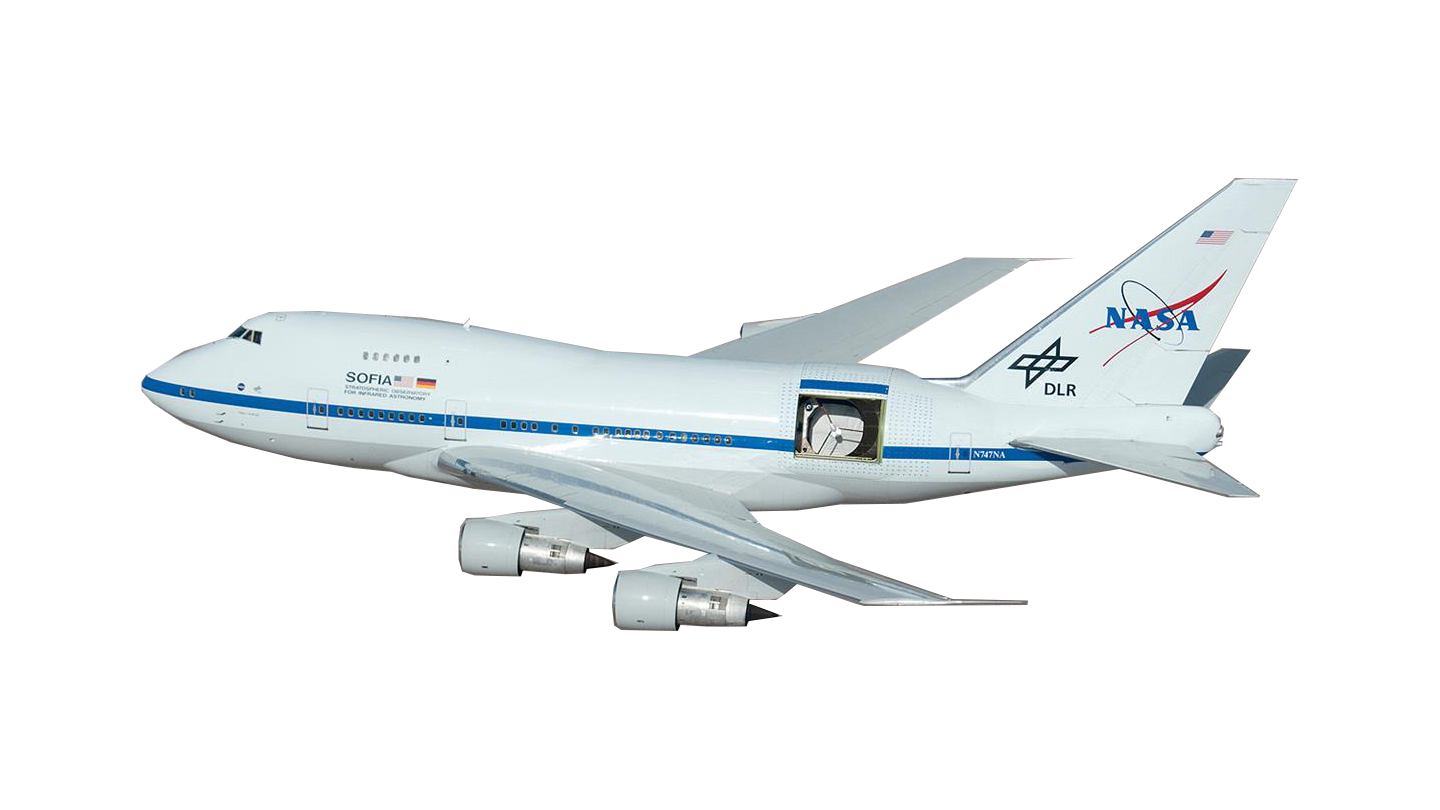
\includegraphics[width=0.7\textwidth]{../test/sofia}\\
\vspace{2.cm}
\textbf{\sl\Large Obs Cycle: OC8M}\\
\vspace{0.5cm}
\textbf{\Large Flight name: MAXINE}\\
\vspace{0.5cm}
\textbf{\Large SOFIA flight: 0}\\
\vspace{0.5cm}
\textbf{\Large FIFI-LS flight: 0}\\
\vspace{0.5cm}
\textbf{\Large Date: 2021-06-05}\\
\vfill
\end{center}
\end{titlepage}
\section{Definitions \& Parameters}
\begin{table}[ht]
\large
\begin{center}\begin{tabular}{ll}
\hline
\hline
\noalign{\vskip 2mm}
Chop angle in J2000 & \textbf{Counter}clockwise from North\\
FOV angle in J2000 & \textbf{Counter}clockwise from North (blue)\\
\noalign{\vskip 2mm}
\hline
\hline
\noalign{\vskip 2mm}
Focus Position (xml) & 372~mm\\
Focus Relation & 4.3 $\mu$m secondary move is -1mm Focus point move\\
Blue bias Voltages & 75~mV\\
Red bias Voltages & 60~mV\\
Chopper Phase & 356$^o$\\
D130/D105 switch blue M2 & [OIII]51.815$\mu$m + 5000~km/s\\
Blue grating switch positions & Home/far: 44000/1910000 induct\\
Red grating switch positions & Home/far: 37000/1753000 induct\\
Blue spexel size & 800 induct\\
Red spexel size & 730 induct\\
\noalign{\vskip 2mm}
\hline
\hline
\noalign{\vskip 2mm}
TO: \hspace{2.2cm} Focus at & 0 $\mu$m\\
\noalign{\vskip 2mm}
KOSMA: \hspace{1.3cm} Setpoint: & --X: -5.3~arcsec\\
& --Y: -7.3~arcsec\\
\noalign{\vskip 2mm}
TEL\_hardware\_status:&Instr\_rotator\_axis\_x = -0.096~mm\\
& Instr\_rotator\_axis\_y = -1.057~mm\\
In Rx\_hardware\_status [mm]:&\\
\hspace{3cm} BD130 &Rx\_cx[2] =  0.90,  Rx\_cy[2] = -0.74\\
\hspace{3cm} BD105 &Rx\_cx[1] =  1.41,  Rx\_cy[1] = -0.60\\
\hspace{3cm} Red   &Rx\_cx[0] = -0.77,  Rx\_cy[0] = -0.69\\
\noalign{\vskip 2mm}
K-Mirror 0 Position: &52~steps\\
\hline
\hline
\end{tabular}
\end{center}
\end{table}
\section{Flight Plan}
\begin{center}
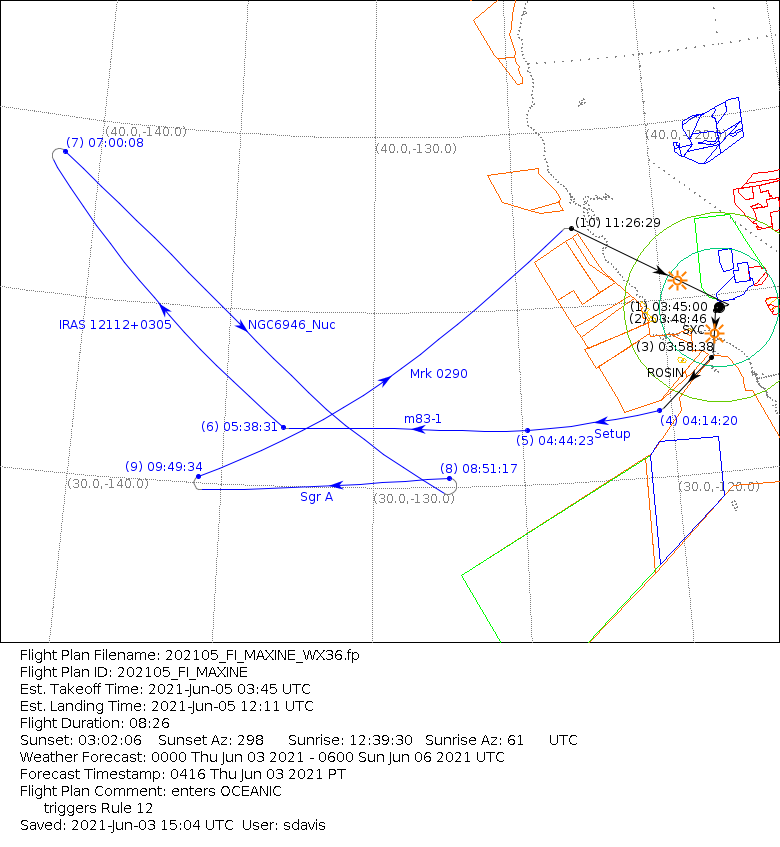
\includegraphics[width=0.70\textwidth]{../test/202105_FI_MAXINE_WX36.png}
\end{center}
\begin{table}[h]
\begin{center}
\begin{tabular}{cccccccr}
\hline
\hline
Leg & Target & Obs Block & Pr & Elevation & UTC start & Duration & Altitude\\
\hline
\hline
1  & Departure &  &  &  & 03:45:00 & 00:02 & 10 Kft\\
2  & Climb &  &  &  & 03:48:46 & 00:08 & 35 Kft\\
3  & Climb &  &  &  & 03:58:38 & 00:14 & 36 Kft\\
4  & Setup &  &  & 24.3-25.0 & 04:14:20 & 00:30 & 38 Kft\\
5  & m83-1 & 70\_0808\_02 & C & 28.3-28.4 & 04:44:23 & 00:53 & 39 Kft\\
6  & IRAS 12112+0305 & 08\_0095\_07 & C & 54.4-43.4 & 05:38:31 & 01:17 & 39/35/41 Kft\\
7  & NGC6946\_Nuc & 09\_0198\_01 & B & 32.6-44.5 & 07:00:08 & 01:45 & 41/75/43 Kft\\
8  & Sgr A & 71\_0024\_14 & C & 30.3-31.1 & 08:51:17 & 00:54 & 43 Kft\\
9  & Mrk 0290 & 08\_0226\_04 & D & 54.8-42.1 & 09:49:34 & 01:35 & 43 Kft\\
10 & Arrival &  &  &  & 11:26:29 & 00:45 & 43 Kft\\
   & Landing &   &  &   & 12:11:52 &   & 0 Kft\\
   & Total flight time &   &  &   &  & 08:26 & \\
\hline
\hline
\end{tabular}
\end{center}
\end{table}
\section{FIFI-LS GTO Cycle 7}
{\large {\bf AOR ID:} 70\_0808 {\bf PI:} Alfred Krabbe}\\
{\bf Comments:}  122 minutes requested in DCS;  120 minutes planned in DCS;  54 of 120 minutes in this series;  66 on MARIO;  54 on MAXINE (this flight)\\
\newline
FIFI-LS GTO Cycle 8
\section{Are local ULIRGs low in metals? Testing a new metallicity diagnostic with FIFI-LS.}
\sectionmark{Are local ULIRGs low in metals? Testing a new metallicity diagnostic w...}
{\large {\bf AOR ID:} 08\_0095 {\bf PI:} Jingzhe Ma}\\
{\bf Comments:}  70 minutes requested in DCS;  70 minutes planned in DCS;  70 of 70 minutes in this series\\
\begin{center}
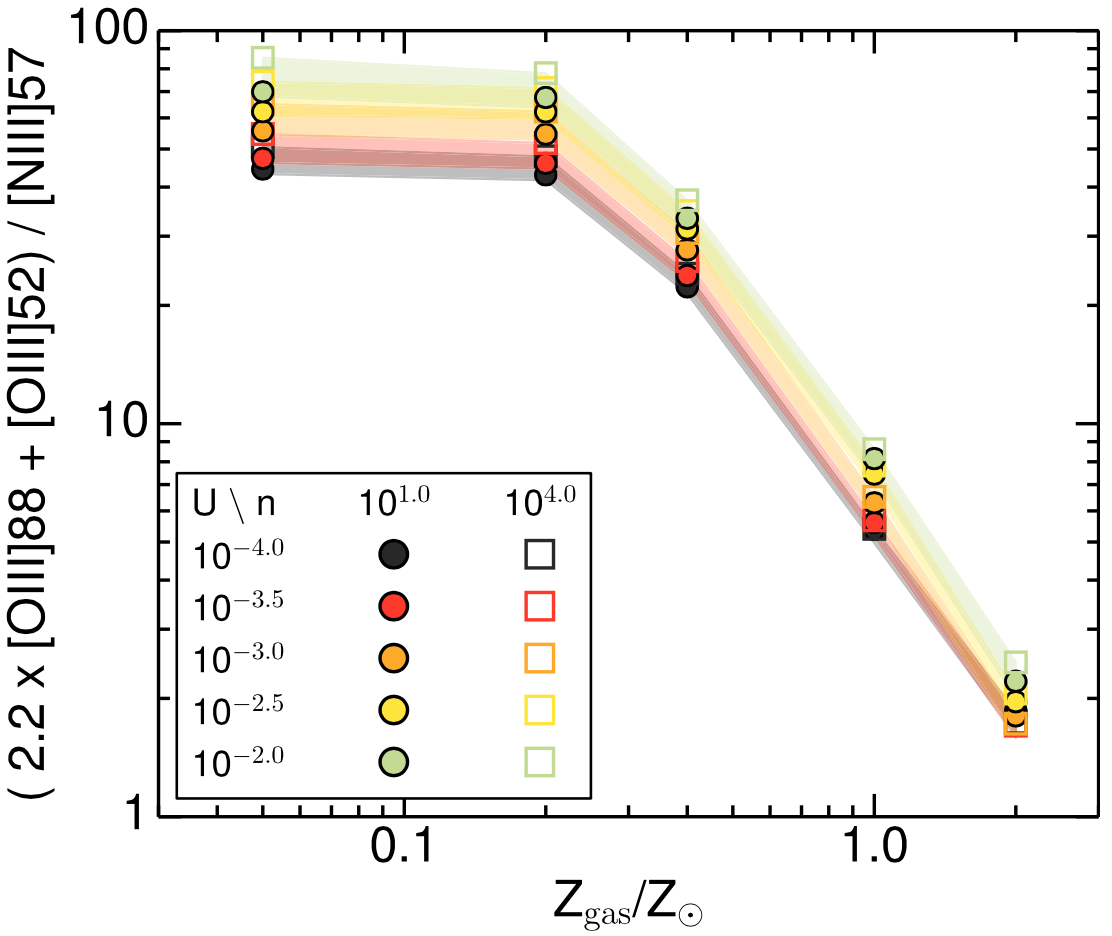
\includegraphics[width=0.60\textwidth]{../test/08_0095/1.png}
\end{center}
A comprehensive study of the physical properties of low-z ultra luminous infrared galaxies (ULIRGs), specifically their interstellar medium (ISM), is critical to understanding the evolution of $>$L* galaxies and active galactic nuclei across cosmic time. ULIRGs at low redshifts are central to this endeavor, as they establish a baseline from which to measure evolution with redshift in the ULIRG population. We propose FIFI-LS observations of the far-IR (FIR) fine structure lines of 11 ULIRGs selected by IRAS at 0.01 $<$ z $<$ 0.13, primarily targeting the [OIII]52 and [NIII]57 um lines, which are currently only accessible by FIFI-LS. The proposed observations will provide comprehensive diagnostics of the physical conditions of the ISM such as the gas density, radiation field intensity, and metallicity that is much less susceptible to extinction than traditionally used UV/optical transitions. We will be able to apply the excellent FIR metallicity diagnostic, ([OIII]52+2.2[OIII]88)/[NIII]57, for the first time, which breaks the density degeneracy and reduces the scatter in the correlation to within 0.2 dex. The unprecedentedly reliable metallicity measurements will address whether ULIRGs lie below the mass-metallicity relation of star-forming galaxies as previously thought based on optical metallicity diagnostics. Along with archival Herschel/PACS+SPIRE observations, we will be able to test all the line-ratio diagnostics by comparing to models (e.g. Cloudy) and identify the best pairs to optimize future observations with ALMA for high-z analogs. This pilot SOFIA program will open up the opportunity to increasing the sample of low-redshift (0.1 $<$ z $<$ 0.3) ULIRGs with the full set of FIR line observations by a factor of 2-3. This program will also demonstrate a key science program for the Origins Space Telescope that focusses on metallicity measurements out to z of 6 with results from Cycle 8 potentially making an impact in Astro2020 Discussions.
\section{Securing Far-Infrared Metal Abundances in NGC 6946}
{\large {\bf AOR ID:} 09\_0198 {\bf PI:} Cody Lamarche}\\
{\bf Comments:}  711 minutes requested in DCS;  406 minutes planned in DCS;  100 of 245 minutes in this series;  50 on MADDILYN;  50 on MATTHEW;  100 on MAXINE (this flight);  45 on MIRIAM\\
\begin{center}
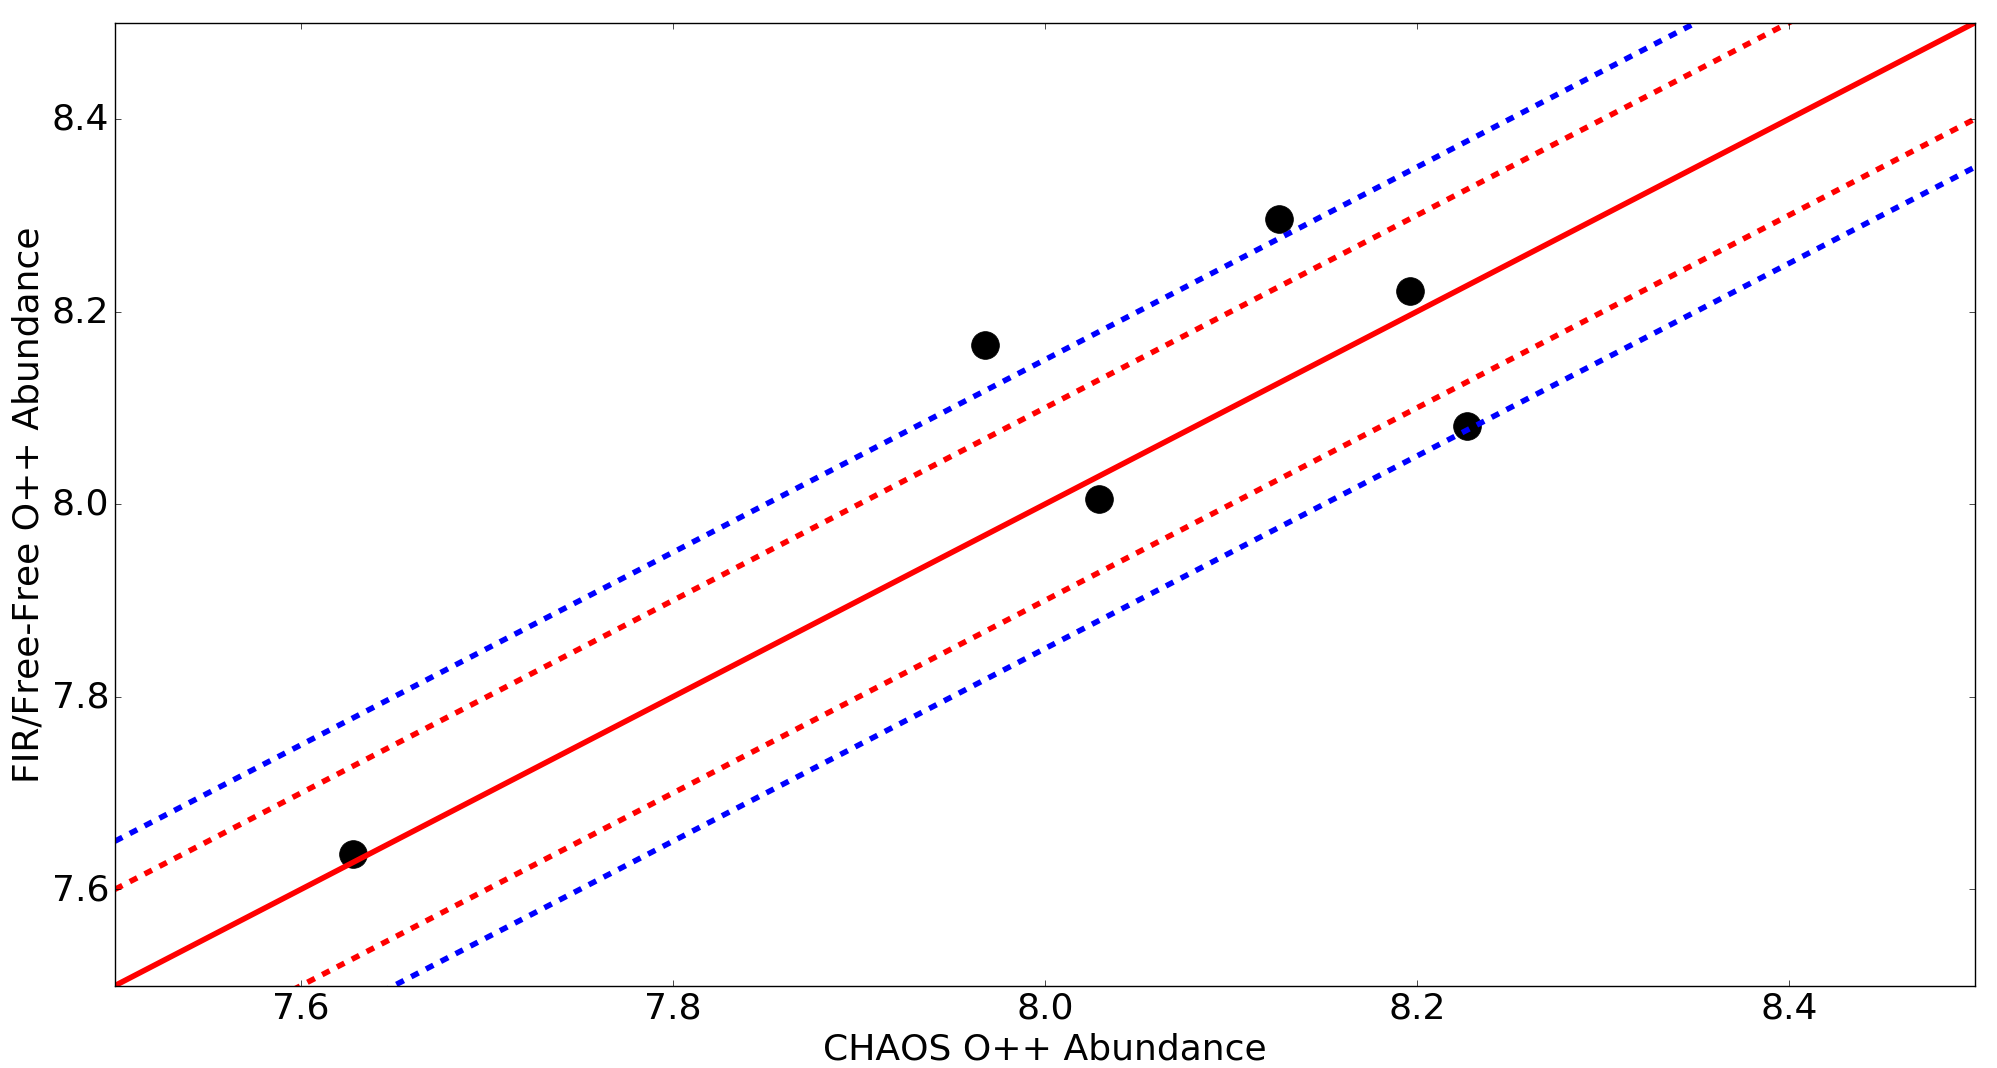
\includegraphics[width=0.60\textwidth]{../test/09_0198/1.png}
\end{center}
Elements heavier than helium contribute less than one percent to the total mass of the local Universe, yet they significantly affect the way in which stars and galaxies form and evolve. Therefore, understanding the chemical enrichment history of the Universe is an essential part of understanding galaxy evolution. The ground-state fine-structure levels of the abundant metals oxygen and nitrogen, accessible to SOFIA in the far-infrared, will play a major role in uncovering this history. With the ability to penetrate the significant dust columns present in galaxies during the peak epoch of cosmic star formation, and little sensitivity to the unknown temperature structure of ionized nebulae that has plagued traditional optical strong-line metal-abundances for decades, FIR abundances offer many powerful advantages. Yet substantial work is still needed locally before these FIR methods can be extended to high-redshift galaxies. We propose a program to study NGC 6946, a bright, metal-rich, nearby spiral galaxy, targeting 8 HII regions that will be observed in concert with the ongoing CHAOS program on the LBT -- the largest, deepest survey of direct spectroscopic optical auroral-line metal-abundances ever undertaken in the local Universe. Combining SOFIA/FIFI-LS with CHAOS spectroscopy, archival Herschel/PACS and Spitzer/IRS, and VLA free-free continuum observations of the targeted HII regions in NGC 6946, we will explore several interrelated temperature-insensitive infrared abundance tools, including direct [OIII] abundances normalized to hydrogen using recombination or free-free emission, and expand and validate the novel O3N3 pure FIR-line abundance diagnostic. Our ancillary data also include deep optical IFU spectral mapping data, which bridge the resolution divide between the SOFIA and ground-based optical surveys.

\section{Instrument Characterization Request: OTF Mapping for FIFI-LS}
{\large {\bf AOR ID:} 71\_0024 {\bf PI:} Christian Fischer}\\
{\bf Comments:}  53 minutes requested in DCS;  53 minutes planned in DCS;  53 of 53 minutes in this series\\
\newline
We propose to test the possibility of implementing an OTF raster mapping mode for FIFI-LS. This mode will be almost identical to that used by the GREAT instrument and to take full 
advantage of the common KOSMA translator interface. We estimate this mode could increase the efficiency of large mapping done with FIFI-LS in total power mode by about 30%. In addition, it would result in much finer spatial sampling, which is clearly beneficial for FIFI-LS observations with its large (6” in the blue and 12” in the red) spaxels. In order to avoid undersampling the PSF with the large pixel scales, most FIFI-LS science observations are obtained in the chop-nod mode with multiple dither positions.  Such observations can be challenging for short 
integrations on large maps. In addition, OTF mapping will result in better self-flat-fielding of the data, since more FIFI-LS spaxels will integrate on the same positions on the sky. In 
summary, OTF mapping with FIFI-LS would greatly improve the data obtained with the instrument by improving the flat-fielding and spatial sampling, enable rapid mapping of large sources, avoid the difficulties of finding nearby chop positions without emission, and simultaneously increase observing efficiency by reducing the telescope overheads
\section{Star-formation efficiencies in nearby, optically luminous Quasars}
{\large {\bf AOR ID:} 08\_0226 {\bf PI:} Andreea Petric}\\
{\bf Comments:} FFI guided;  129 minutes requested in DCS;  150 minutes planned in DCS;  75 of 108 minutes in this series;  75 on MAXINE (this flight);  33 on MILDRED\\
\begin{center}
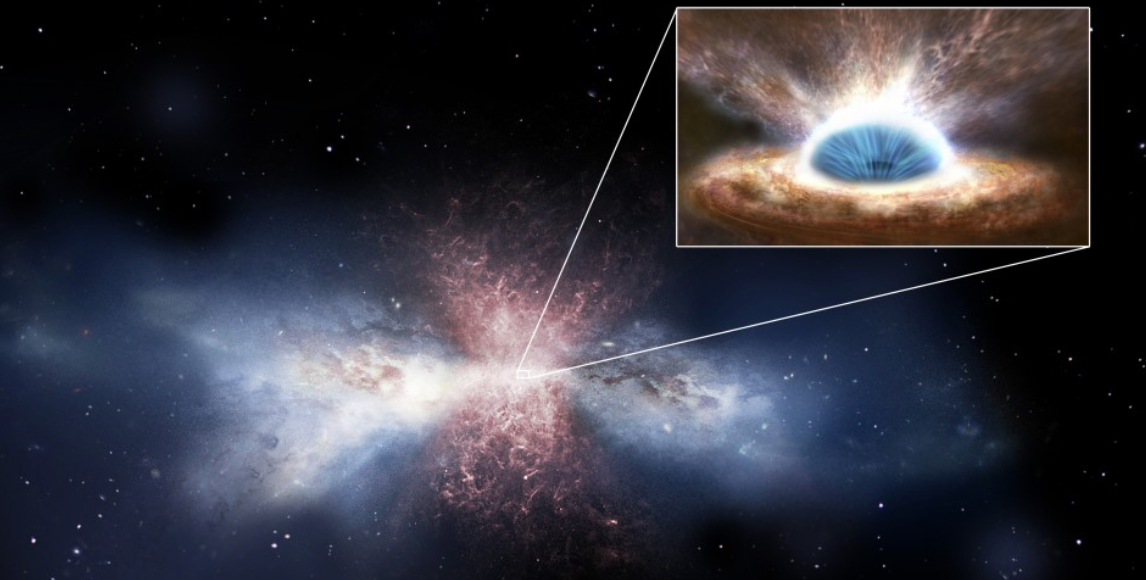
\includegraphics[width=0.60\textwidth]{../test/08_0226/1.png}
\end{center}
Most bulge-dominated galaxies have at their centers black holes with masses that tightly correlate with the masses of their hosts' bulges. This may indicate that the black holes may regulate galaxy growth, or vice versa, or that they may grow in lock-step. The quest to understand how, when, and where those black-holes formed motivates much of extragalactic astronomy. The [CII] 157.74 micron fine structure line of singly ionzed carbon has been calibrated  both as a measure of star-formation rates and as a way to estimate the star-formation efficiencies. Recent SOFIA observations of  [CII] in nearby low-luminosity AGN suggest that: high ratios of [CII] to FIR may be associated with obscured AGN outflows and that the [CIII] may be at the interface between warm and cold gas in those outflows. The observations we propose here will test whether luminous, obscured AGN have higher [CII]/FIR ratios than luminous, non-obscured AGN.

\end{document}